\documentclass{bioinfo}
\usepackage{epstopdf}
\usepackage{url,color}
\copyrightyear{2015}
\pubyear{2015}

\usepackage{subfigure,bm,algorithm,algorithmic,color,subfigure}
\def \M {\mathcal{M}}
\def \x {\mathbf{x}}
\def \R {\mathbb{R}}
\def \D {\mathcal{D}}
\def \xh {\widehat{\x}}
\def \f {\mathbf{f}}
\def \P {\mathbf{P}}
\def \ab {\boldsymbol \alpha}
\def \X {\mathcal{X}}
\def \E {\mathrm{E}}
\def \z {\mathbf{z}}
\def \L {\mathcal{L}}

\newtheorem{thm}{Theorem}

\usepackage{citesort}
\usepackage{pslatex}
\usepackage{epsfig}
\usepackage{epsf}
\usepackage{amsmath, amsthm, amssymb, multirow, paralist, subfigure}
\usepackage{graphicx}


\begin{document}

\firstpage{1}

\title{Towards Measuring Plant Photosynthetic Heterogeneity}
\author[Tessmer \textit{et~al}]{Oliver L Tessmer\,$^{1}$, Xi Yin\,$^{1}$, Jeffrey A Cruz\,$^{2,3}$, Linda J Savage\,$^{2}$, Xiaoming Liu\,$^{1}$, David M Kramer\,$^{2,3~\ast}$, Jin Chen\,$^{1,2}$ \footnote{to whom correspondence should be addressed}}
\address{$^{1}$Department of Computer Science and Engineering, Michigan State University, East Lansing, MI 48824, USA\\
$^{2}$Department of Energy Plant Research Laboratory, Michigan State University, East Lansing, MI 48824, USA\\
$^{3}$Department of Biochemistry and Molecular Biology, Michigan State University, East Lansing, MI 48824, USA}

\history{Received on XXXXX; revised on XXXXX; accepted on XXXXX}

\editor{Associate Editor: XXXXXXX}

\maketitle

\begin{abstract}

\section{Motivation:} Photosynthesis is one of the most important biological processes on earth. Plant photosynthetic heterogeneity refers to a plant comprising multiple regions, many of which have significantly different photosynthesis properties, probably because of vastly different leaf developmental stage and tolerance level to environmental changes. Measuring plant photosynthetic heterogeneity enables biologists to interpret the sophisticated photosynthesis phonemics data, which is particularly important for plant primary productivity estimation and modeling.

\section{Results:} Taking advantage of the rapid developing non-invasive plant phenotyping technologies, we develop a new plant photosynthetic heterogeneity measurement called PlantPH to effectively identify and integrate the plant morphological and physiological features.

The application of PlantPH on more than 1,000 Arabidopsis chloroplast plants, including dozens of ecotypes and hundreds of chloroplast mutant strains, has successfully identified a group of genes that affect photosynthesis under simulated natural environments.

\section{Availability:}
Software is available at XXX.

\section{Contact:} \href{jinchen@msu.edu}{jinchen@msu.edu}, \href{kramerd8@cns.msu.edu}{kramerd8@cns.msu.edu}
\end{abstract}

\section{Introduction}

%[Phenotyping]
By consuming water, light and $CO_2$, plants produce sugars and release $O_2$ with photosynthesis \citep{kramer2011importance}. The process involves the formation of high energy intermediates capable of generating reactive oxygen species. The photosynthetic apparatus, chloroplast and surrounding leaf tissue is inherently susceptible to oxidative damage, especially under stress conditions when the supply of light energy exceeds the capacity to utilize it \citep{durrant1990characterisation,asada1996radical}. Plants have evolved a number of mechanisms, such as photosynthetic apparatus damage and repair \citep{melis1999photosystem}, to dissipate excess light energy to minimize the potential for damage at the expense of photosynthetic efficiency \citep{adams2006energy,rochaix2014regulation}. However, these mechanisms are sensitive to leaf development and thus may change from one leave tissue to another, resulting in heterogenous photosynthetic patterns (see examples in Figure \ref{fig:heterogeneityexample} where the chlorophyll fluorescence images are false-color images and the light intensity of every pixel is proportional to photosynthetic efficiency~\citep{toet1996new}). The heterogeneous patterns may also vary with the position, size and growth rate of leaves, since leaves at the same node \textcolor{red}{are} %is 
unique in age. By integrating plant morphological and physiological features, measuring plant photosynthetic heterogeneity aids interpretation of %the 
sophisticated photosynthesis phonemics data, \textcolor{red}{which is} particularly important for plant primary productivity estimation and modeling \citep{meng2007spatial}.

\begin{figure}[tb]
\centering
\subfigure[\scriptsize Ecotype Italy]{\includegraphics[width=0.35\linewidth]{example1.PNG}}~~~~~~~~~~
\subfigure[\scriptsize Ecotype Sweden]{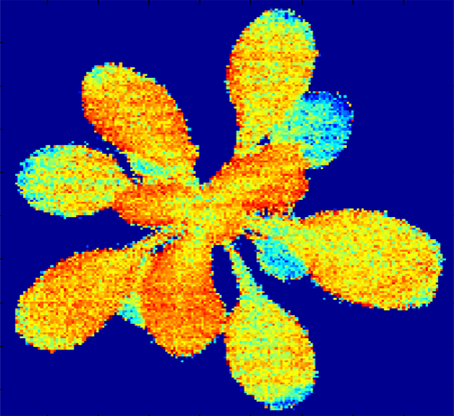
\includegraphics[width=0.35\linewidth]{example2.PNG}}\vspace{-0.05in}
\subfigure[\scriptsize Histogram of all leaves in (a)]{\includegraphics[width=0.4\linewidth]{example1-hist.PNG}}~~~
\subfigure[\scriptsize Histogram of all leaves in (b)]{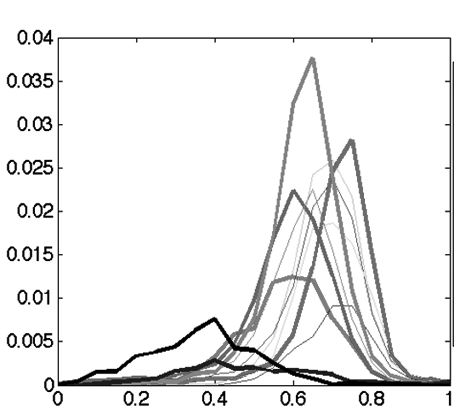
\includegraphics[width=0.4\linewidth]{example2-hist.PNG}} \vspace{-0.2in}
%\subfigure[Gene ontology (biological process)]{\includegraphics[width=0.31\textwidth]{eva_bp.eps}}
\caption{\scriptsize We demonstrate the photosynthesis heterogeneity using two Arabidopsis ecotypes (Italy and Sweden). Both plants were grown under the same stress conditions, but the false-color images of photosystem II activity (a,b) and the distributions of the leaf-level photosynthesis (c,d) show that the Italy ecotype is more suspectable to environmental changes. \vspace{-0.3in} } \label{fig:heterogeneityexample}
\end{figure}


%Advanced technologies in high-throughput plant photosynthetic phenotyping (the Dynamic Environment Photosynthesis Imager, or DEPI) have been developed \citep{cruz2014depi,houle2010phenomics}. These systems generate huge amount of images of plant photosynthesis that can be used to quantify photosynthetic behavior in genetically diverse populations, leading to better understanding of the underlying mechanisms that control the photosynthetic properties \citep{fiorani2013future,rascher2011non}, enabling to measure variability in various photosynthetic parameters at high resolution across leaves.

%The model of spatial heterogeneity of the photosynthetic properties may reveal $CO_2$ intake capability, stomatal conductance and tolerance level to environmental changes of leaf tissues at different developmental stages.

%photosynthetic heterogeneity refers to a plant comprising multiple regions, a significant amount of which have different photosynthesis properties, %. %For example, under full sunlight photosynthesis usually captures at most only of available energy (bonner1962upper, von1981some, kramer2011importance).

Heterogeneity is a statistical concept relating to the uniformity in a substance~\citep{hall2003interpretation}. The granularity of %the 
plant photosynthetic heterogeneity studies can range from cells to tissues, leaves, and even to the whole plant level. While in-leaf variability in photosynthetic activity has been well-studied for the understanding of the effects of stomatal conductance~\citep{Cheeseman1991,Buckley1997}, recent works show that photosynthetic capacity may decline with vertical gradient and leaf age \citep{Kitajima2002,chen2008effect}, suggesting that leaf-based photosynthetic heterogeneity is a key towards processing and understanding photosynthesis phenotype images. % the understanding of plant photosynthesis.

%The leaf 
\textcolor{red}{Leaf} heterogeneity in photosynthesis was \textcolor{red}{first} %firstly been 
studied  with computer simulation~\citep{chen2008effect}. Due to the lack of high-throughput phenotyping technologies, the authors determined the effects of biochemical variability via the Farquhar model (a mechanistic, biochemical model widely used to describe steady-state $CO_2$ assimilation in leaves), incorporating defined degrees of spatial variability of its parameters~\citep{sharkey1985o2,farquhar2001models}. %The results showed that spatial heterogeneity in photosynthesis can affect the ability of the Farquhar model to accurately characterize photosynthesis at the leaf level~\citep{chen2008effect}.
%
Recently, with the advent of advanced technologies of biomedical imaging, directly measuring heterogeneity has recently assumed new importance~\citep{tiihonen1996cerebral,wieneke1999non,wang2000,cruz2014depi}. The rapid development of lighting and imaging techniques enables real-time non-invasive monitoring of photosynthesis \citep{houle2010phenomics,cruz2014depi}, resulting in vast amount of chlorophyll fluorescence images of plants \citep{wituszynska2013multivariable}. These images can be used to quantify photosynthetic behavior in genetically diverse populations, enabling \textcolor{red}{the measurement of} %to measure 
variability of photosynthetic parameters at high resolution across leaves, leading to better understanding of the underlying mechanisms that control the photosynthetic properties \citep{rascher2011non,fiorani2013future}. %However, there is no

Measuring leaf-based photosynthetic variability in large-scale phenotyping experiments requires automatic%al 
identification of most of the visible leaves in all fluorescence images and an appropriate measurement for the variation of photosynthesis parameters across leaves that takes geometrical (leaf position and size), temporal (leaf growth rate) and physiological (leaf age) information into consideration. However, there is currently no existing infrastructure to analyze such \textcolor{red}{an} amount of phenotype information. %The challenges of this work include not only the accurate leaf alignment in complex plant leaf layout, but also the development of a new heterogeneity measure that
%
In this paper, we present a new computational framework called {\it Plant Photosynthesis Heterogeneity} (PlantPH), and use the tool to analyze the leaf-level photosynthesis heterogeneity patterns of more than 100 Arabidopsis chloroplast mutant strains over dynamic lighting conditions, each with at least four replicates. The followed outlier detection process successfully \textcolor{red}{identifies} %identify 
mutants with distinct heterogeneity patterns under specific subsets of the environmental conditions.
%
Overall, PlantPH has the following three advantages: %The mutant screen analysis reveals that ...
\begin{enumerate}\vspace{-0.1in}
  \item~~It is the first computational framework to measure plant leaf-level heterogeneity of photosynthesis with leaf size, position and growth rate.
  \item~It's performance is significantly better than %the 
traditional heterogeneity tests that cannot fully use the spatial and temporal information in the fluorescence images.
  \item~It discovers multiple types of photosynthetic variabilities in a large scale experiment.
\end{enumerate}

%Comparing with the existing heterogeneity approaches, our method is novel in the following ways:
%
%1.	PlantPH
%
%2. PlantPH models heterogeneity ..
%
%3. PlantPH refers to the differences between individual leaf photosynthesis and the pooled photosynthesis across all the leaves, with the weights being those used in the pooling method. With PlantPH, transient regional variation events that do not affect the whole plant photosynthesis, can be easily discovered.


%, in which hundreds of plants are screened simultaneously,
\vspace{-0.2in}
\section{Background}
The inputs to plant heterogeneity test are leaf-level photosynthesis values obtained using leaf segmentation methods. The general method of assessing whether the leaves of a plant are photosynthetically homogeneous or heterogeneous is by means of the Cochran's Q-test \citep{conover1999Practical} and the $I^2$ statistic \citep{higgins2002quantifying,higgins2003measuring}.


%The process has three steps.
%
%In short, the Cochran's Q-test is computed by summing the squared deviations of each object's effect estimate from overall effect estimate, weighting the contribution of each object's effect estimate by its inverse variance \citep{conover1999Practical}.
%
%The $I^2$ statistic measures the extent of true heterogeneity dividing the difference between the Cochran's Q-test value and its degree of freedom by the Q-test value \citep{higgins2003measuring,higgins2002quantifying}.
%


%and none of them can take plant specific information, such as leaf position, into the heterogeneity measurement.

%We have developed a new leaf segmentation approach called PlantPH to identify leaves from photosynthesis images...





%---------------------------
%\section{Background}

%\vspace{-0.2in}
\subsection{Leaf Alignment and Tracking}\label{sec:alignment}

The input to Plant heterogeneity test are leaf-level photosynthesis values. To obtain the values, a method is needed to identify every piece of leaf from a whole plant image, measure the florescence intensity of every pixel on a leaf, and finally convert the intensity values to biologically meaningful photosynthesis parameters.

In our previous studies, we have developed a new multi-leaf alignment and tracking algorithm~\citep{yin2014} to meet the requirements.  %[MORE INTRO TO LEAF ALIGNMENT HERE]
%
Different from the naive procedure of aligning leaves iteratively using the Chamfer distance~\citep{barrow1977parametric}, our tool aims to find the best alignment of multiple leaves simultaneously in an input image. We formulate an optimization problem of an objective function with three terms: the average of chamfer distances of aligned leaves, the number of leaves, and the difference between the synthesized mask by the leaf candidates and the original image mask.
%
The extension on leaf tracking~\citep{xi2014tracking} tracks multiple leaves from fluorescence plant videos by continuously applying template transformation to the current leaf candidates in order to fit to the previous frame.
%
Experimental results show that the multi-leaf alignment and tracking tool performs substantially better than the baseline of the Chamfer matching algorithm in terms of both accuracy and efficiency.

%Differences between individual leaves with similar photosynthetic efficiency can be subtle, making the boundaries between them difficult to define and creating a significant challenge for subsequent shape analysis. The difficulty even arises when individual leaves overlap and occlude one another in these false-color images.

%We have developed a framework based on the well-known Chamfer Matching algorithm \citep{yin2014}. Multi-leaf alignment aims to segment all leaves with pre-defined leaf templates and estimate the two tip points of each leaf. The tracking algorithm consists of two steps. First, a set of leaf templates are applied to the target image to generate the same amount of leaf candidates. Second, we adopt multi-objective optimization to select a subset of leaf candidates. The objective is to select a minimal number of leaf candidates with smaller Chamfer distances to cover the test image mask as much as possible.




However, there are two obstacles preventing us from directly using our leaf alignment algorithm in PlantPH. First, the tool only identifies one leaf if the leaf overlap rate is high (e.g. 59\%).
%
In addition, the leaf boundaries are not precisely identified by the multi-leaf alignment tool, since predefined leaf templates are used.
%
Subsequently, the leftover of leaf alignment consists of partial leaves that are highly overlapped and leaf boundaries of the successfully recognized leaves (Fig. XX). The covered leaves are usually old leaves with diverse photosynthesis activities. Simply deleting them may result in inaccurate heterogeneity scores.
%
The second obstacle is that the leaf alignment process is a time consuming process. Processing 100 images each containing 20 plants may take about 5 hours. It is not practical to apply leaf alignment on all the images (in our case 17.8 years are need to process all the 31,120 images).

\vspace{-0.2in}
\subsection{Heterogeneity Test}

Cochran's Q-test is the classical measure of heterogeneity~\citep{conover1999Practical}. In the scenario of leaf-based photosynthetic heterogeneity, $Q$ is calculated as the weighted sum of squared differences between the photosynthesis value of an individual leaf and the pooled photosynthesis value across all leaves with the weights being those used in the pooling method. The distribution of $Q$ is a chi-square statistic with $k-1$ degrees of freedom, where $k$ is the number of leaves. Cochran's Q-test has been widely used in biomedical studies. For example, heterogeneity in the aggressiveness of tumor cell populations has been adopted as an essential feature in predicting treatment success~\citep{OSullivan2003}. %However, due to the nature of plants, leaf-based photosynthetic heterogeneity often includes a small number of leaves, and thus the power of the Q-test in such circumstances could be low~\citep{higgins2003measuring, gavaghan2000evaluation}.
%
%Conversely, Q has too much power as a test of heterogeneity if the number of leaves is large \citep{higgins2003measuring}.
%
%An additional test is provided with the odds ratio meta-analysis \citep{breslow1987statistical}. It is arguably not possible to examine the null hypothesis that all studies are evaluating the same effect, by considering the only the summary data from the studies: The heterogeneity test results should be considered alongside a qualitative assessment of the combinability of studies in a systematic review.

The $I^2$ statistic describes the percentage of variation across studies that is due to heterogeneity rather than chance~\citep{higgins2002quantifying,higgins2003measuring}. $I^2$ can be calculated as $I^2 = (Q - df)/Q$, where Q is Cochran's Q-test heterogeneity statistic and $df$ is the degrees of freedom. A negative value  indicates no observed heterogeneity, and larger values show increasing heterogeneity. $I^2$ is an intuitive and simple expression of the inconsistency. $I^2$ of leaf-based photosynthetic heterogeneity does not inherently depend upon the number of leaves, so that $I^2$ values of different plants become comparable. A confidence interval for $I^2$ can be constructed using either the iterative non-central chi-squared distribution method \citep{hedges2001power} or the test-based method \citep{higgins2002quantifying}.

However, due to the nature of plants, leaf-based photosynthetic heterogeneity often includes a small number of leaves. For example, there are \textcolor{red}{fewer} %less 
than ten rosette leaves %of
\textcolor{red}{on a} 2-3 week old Arabidopsis thaliana (a model plant). Thus, the power of the traditional Cochran's Q-test and $I^2$ statistic in such circumstances is low~\citep{higgins2003measuring, gavaghan2000evaluation,huedo2006assessing,ioannidis2007uncertainty}.

Furthermore, leaves with different locations, sizes or growth rates may have diverse photosynthetic performance, resulting in high level of heterogeneity~\citep{van1991insertional,chen2008effect}. But none of these factors has yet been taken into the existing measurement of heterogeneity.



%To measure leaf-based photosynthetic variability in a large-scale phenotyping experiment, in which hundreds of plants are monitored in real time, it is naturally required to identify each leaf from top-view photosynthesis images automatically. However, leaf identification is a difficult task, in that 1) all the leaves are very similar in appearance especially for model plant Arabidopsis; 2) leaf features are much fewer than the well-studied face recognition problem; and 3) leaves may overlapped with each other that makes the problem more complicated. In short, there are two challenging computational problems. First, how to separate overlapped leaves in photosynthesis images where the leaf boundaries are obscure. Second, how to recognize incomplete leafs due to occlusion. Alternatively, approximation approaches can be used to estimate the leaf-based photosynthetic heterogeneity, including distribution based, region based and pixel based approaches. While these approximation approaches are easier to model, their performance may be reduced.

%Based on the rapid development in the fields of bio-imaging and computer vision, we develop a new approach called PlantPH that quantifies the heterogeneity of photosynthesis across leaves of the same plant, and compare the degree of inconsistency among mutant strains in varying environmental conditions.

\begin{figure}
  \centering
  % Requires \usepackage{graphicx}
  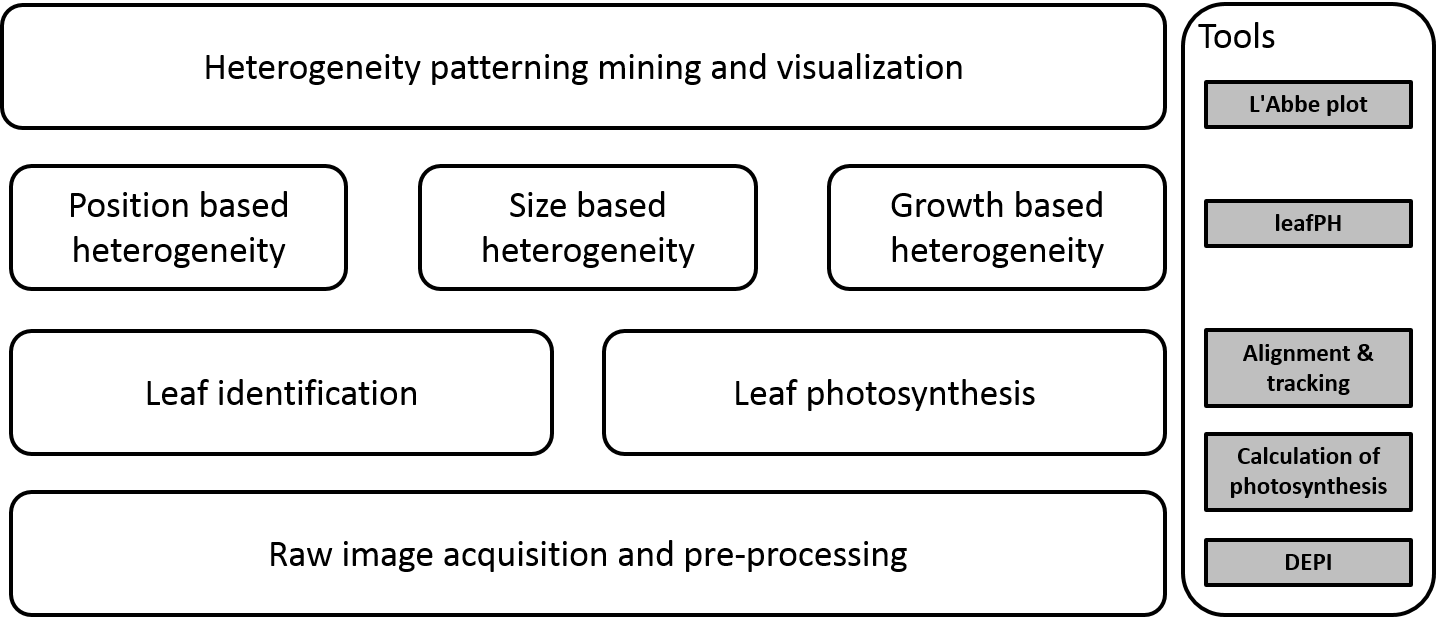
\includegraphics[width=0.45\textwidth]{architecture.png}\vspace{-0.1in}
  \caption{Architecture of plant phenotype analysis where PlantPH serves as a key player for heterogeneity pattern mining.}\label{fig:architecture}\vspace{-0.2in}
\end{figure}

%the effect of heterogeneity

\begin{methods}\vspace{-0.2in}
\section{Method}\label{sec:PlantPH}
In this article, we present a new leaf-based plant phenotype heterogeneity measurement, followed with a workflow to efficiently use the measurement on large-scale experiments (Fig.~\ref{fig:architecture}).

\subsection{PlantPH Measurement}
We introduce a new leaf-based heterogeneity measurement called $PlantPH$ as follows.
%
First, let $T = \{T_{1}, T_{1}, \ldots, T_{n}\}$ be the set of effect estimates of a plant $p$ with $n$ leaves.
The effect estimate $T_{i}$ of leaf $l_i$ in plant $p$ is defined as the difference between the averaged photosynthetic values of the leaf and  the whole plant.
%
Mathematically, in each effect estimate $T_i$, let $u_i$ and $u_p$ be the averaged photosynthesis values of leaf $l_i$ and the whole plant $p$, respectively. Under the assumption of normal distribution and homoscedasticity, the effect estimate $T_i$ is the standardized mean difference \citep{hedges1998fixed}, which can be estimated by: %$T_{i} = c(l_i) (mean(l_i)-mean(p))/S(l_i,p)$ ,
%
\begin{equation}\label{eq:effectestimate}
T_{i} =  \frac{c(l_i)\left(\mu(l_i)-\mu(p)\right)}{S(l_i,p)}
\end{equation}

\noindent where $c(l_i)$ is a correction factor for the positive bias suffered by the standardized mean difference with small sample sizes, which can be estimated by $c(l_i) = 1-3/(4(|l_i|-1)-1)$ \citep{hedge1985statistical}. This adjustment will reduce the effect estimate of small leaves that only have a few pixels, and thus increase the robustness of the heterogeneity model \citep{huedo2006assessing}.
%
%According to the equation of $c(L_i, L_j)$, $c(L_i, L_j)$ is close to 1 for large leaves with many pixels, otherwise it is close to 0, down-weighing the value of heterogeneity.
%
The pooled estimate of the within-group standard deviation $S(l_i, p)$ can be computed with \citep{hedges1998fixed}:
%
\begin{equation}\label{eq:S}
S(l_i, p) = \sqrt{\frac{(|l_i|-1)std^2(l_i)+(|p|-1)std^2(p)}{|l_i|+|p|-2}}
\end{equation}

\noindent where $std^2(l_i)$ is the variance of leaf $l_i$, $std^2(p)$ is  the variance of the averaged values of all leaves in plant $p$, and $|p|$ are the total number of pixels of leaf $l_i$ and the whole plant $p$, respectively.

%The sample variance of $T_{ij}$ is estimated using Equation \ref{eq:ST} \citep{hedges1998fixed}.
%
%\begin{equation}\label{eq:ST}
%ST_{ij} = \frac{|L_i|+|L_j|}{|L_i||L_j|}+\frac{T_{ij}^2}{2(|L_i|+|L_j|)}
%\end{equation}

Then the Cochran's Q-test statistic for determining whether there is true leaf-based photosynthetic heterogeneity among the leaves is defined as:
%
\begin{equation}\label{eq:Q}
%Q=\sum_{i=1}^n \frac{\left(T_i-mean(T)\right)^2}{\tau^2}
Q=\sum_{i=1}^n w_i\left(T_i-\frac{\sum_{j=1}^n w_jT_j}{\sum_{j=1}^n w_j}\right)^2
\end{equation}

\noindent where $n$ is the total number of leaves of the plant $p$,  the right part of the equation is the weighted mean of effect estimates of all the leaves of the plant $p$, and $w_i=1/(\tau^2+\delta_i^2)$, where $\delta_i^2$ is the sampling variance of the effect estimate $T_i$, and $\tau^2$ is the between-study variance of all the effect estimates \citep{huedo2006assessing}.

To estimate $\delta_i^2$, the sampling variance of each effect estimate $T_i$, we use the photosynthetic value of every pixel in the high-resolution florescence images, in which the total number of samples of a plant is much greater than 1000. According to \citep{huedo2006assessing}, $\delta_i^2$ is close to 0. Hence, by ignoring the computation of  $\delta_i^2$ and replacing it with 0, we have:
%
\begin{equation}\label{eq:Q2}
%Q=\sum_{i=1}^n \frac{\left(T_i-mean(T)\right)^2}{\tau^2}
Q=\frac{1}{\tau^2}\sum_{i=1}^n\left(T_i-\frac{\sum_{j=1}^n T_j}{n}\right)^2
\end{equation}

Since both the between-study variance $\tau^2$ and the Q statistic represent the true heterogeneity among the distributions of the leaf-level photosynthesis, we move $\tau^2$ to the left of the equation and define a new measure called $PlantPH$:
%
\begin{equation}\label{eq:Q3}
PlantPH(f)=\sum_{i=1}^n\frac{\left(nT_if(l_i)-\sum_{j=1}^n T_jf(l_j)\right)^2}{n^3}
\end{equation}

In Equation \ref{eq:Q3}, $PlantPH(f)$ is a measure for determining whether there is true heterogeneity among all leaves of a plant. It is independent to the total number of leaves, allowing for being comparable among different plants. We take plant leaf morphology into the plant heterogeneity test by defining $f(.)$ as a function to measure the morphological properties (e.g., the area, position or growth rate) of a piece of leaf.

Specifically, in $PlantPH(area)$ we have $f(l_i)=area(l_i)$, which measures the leaf surface area \citep{boyes2001growth,tessmer2013functional}, and in $PlantPH(growth)$ we define $f(l_i)=growth\_rate(l_i)$ by adopting a three-parameter nonlinear growth model to compute both the absolute growth rate (AGR) and the relative growth rate (RGR) \citep{Richards1959,hunt1982plant,tessmer2013functional}. Moreover, in $PlantPH(position)$, we define $f(l_i)=position(l_i)$ to be 0 if $l_i$ is at the center of the plant, and 1 otherwise, in order to measure whether the leaves with a similar developmental stage have heterogeneous photosynthetic values.

 %we apply the following approach:
%\begin{enumerate}
%  \item Let $f(l_i)$ be $position(l_i)$ which returns 0 if $l_i$ is at the center of the plant, and returns 1 otherwise;
%  \item Compute $PlantPH(position)$ using Equation \ref{eq:Q3};
%  \item Since the above computation considers the plant center, we adjust $PlantPH(position)$ by
%\end{enumerate}

%%
%We estimate $\tau^2$ using the method of moments \citep{dersimonian1986meta}:
%
%\begin{equation}\label{eq:tau}
%\tau^2 = \left\{\begin{matrix}
% \frac{\widetilde{Q}-(n-1)}{\sum \widetilde{w_{i}}-\sum \widetilde{w_{i}}^2/\sum \widetilde{w_{i}}} & \widetilde{Q}>|T|+1\\
% 0 & else
%\end{matrix}\right.
%\end{equation}
%%
%\noindent where $\widetilde{Q}$ and $\widetilde{w_{i}}$ are the results of Q test of fixed effect estimate and the corresponding weight, which is computed as:	
%
%\begin{equation}\label{eq:weight}
%\widetilde{w_{i}} = \frac{1}{std^2(l_i)+c }
%\end{equation}
%
%%[Pos(L_i)\neq  Pos(L_j)] \times
%

\subsection{PlantPH Workflow}

\begin{figure}
  \centering
  % Requires \usepackage{graphicx}
  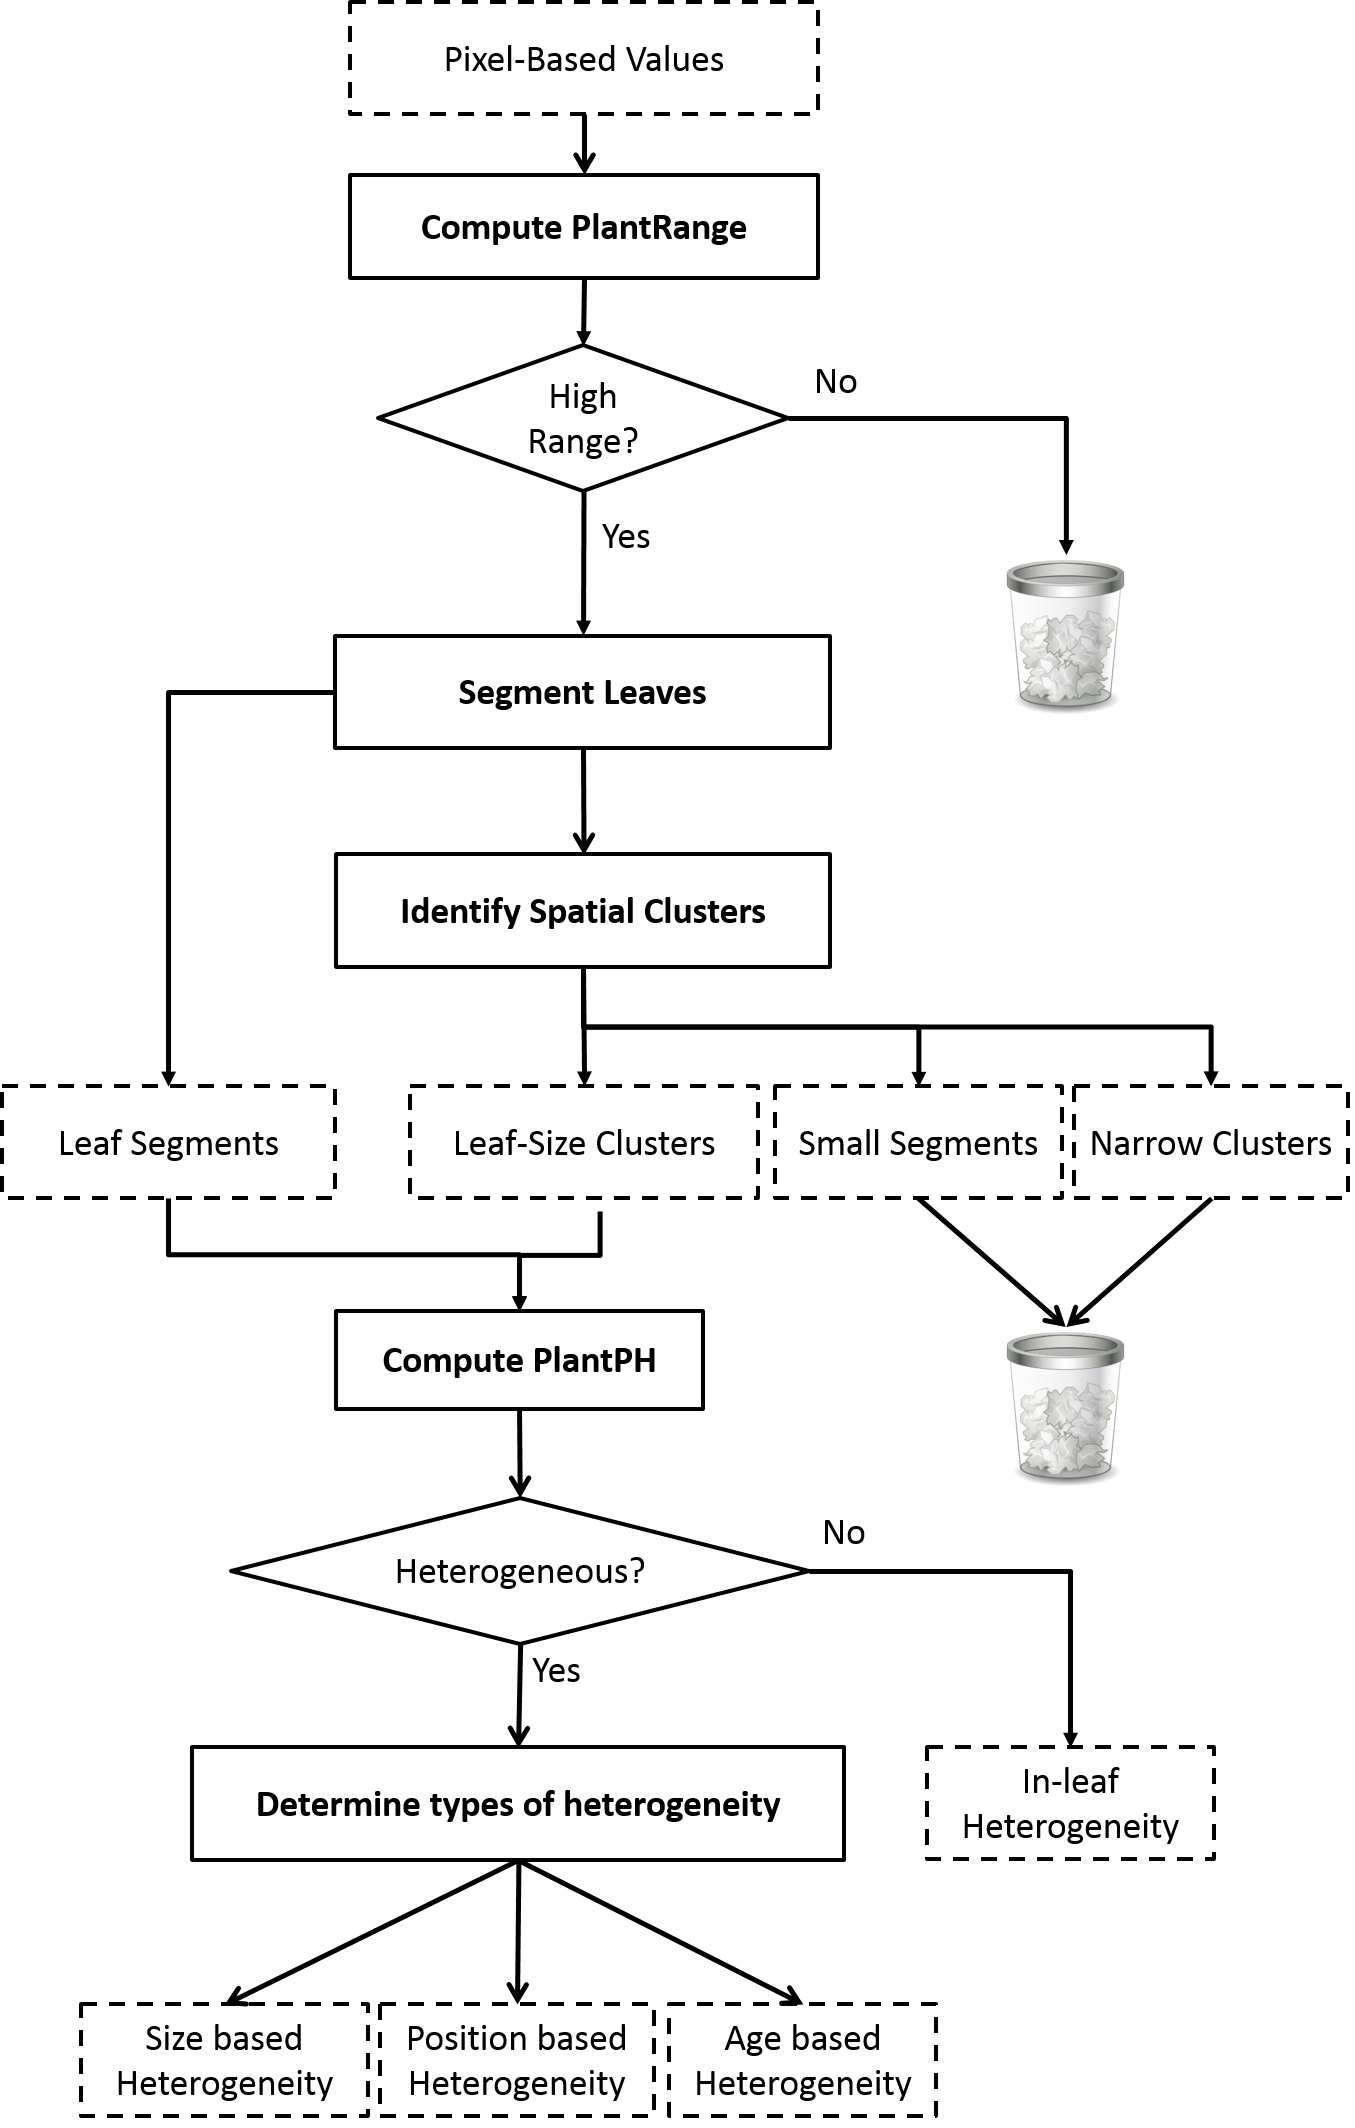
\includegraphics[width=0.45\textwidth]{workflowchart-detail.png}\vspace{-0.1in}
  \caption{Workflow of PlantPH, where the boxes with dashed lines are data and the boxes with solid lines are procedures.}\label{fig:workflow}\vspace{-0.2in}
\end{figure}


As described in Section~\ref{sec:alignment}, it is impractical to directly call leaf alignment algorithms in PlantPH simply because of the high leaf overlap rate and computational efficiency. To meet the gap, we introduce an efficient workflow for leaf heterogeneity test (Fig.~\ref{fig:architecture}).
%
First of all, an efficient statistical method is applied to screen the whole image dataset to identify all the candidate heterogenous plant images. Second, on the candidate set, we apply a leaf alignment and tracking method and a spacial clustering method to identify leaves~\citep{ester1996density,kriegel2011density,xi2014tracking,yin2014}. In addition, a small region is added in the center of every plant image to represent the young leaves that are difficult to identify. Finally, we compute the leaf-based photosynthesis heterogeneity for every plant image using Eq.~\ref{eq:Q3}.
%
%All the pixels not contained in any leaf boundary are considered as an extra leaf. A leaf is ignored if its area is smaller than the plant center circle.

By manually browsing many plant images, we observe that i) heterogeneous plants are rare in the whole dataset, and ii) the distribution of all the photosynthesis values of a homogenous plant usually has a relatively narrower range than that of a heterogenous plant.
%
Therefore, we compute a p-value for the range of photosynthetic values for every image:
%
\begin{equation}
p\_value(PlantRange(p_{it})) =
\end{equation}
\noindent where $PlantRange(p_{it})$ is defined as:
%
\begin{equation}
PlantRange(p_{it}) = max(p_{it}) - min(p_{it})
\end{equation}
%
\noindent where $p_{it}$ is the image of plant $i$ at time $t$, and functions $max$ and $min$ return the maximal and the minimum values of all the photosynthetic values of $p_{it}$ after deleting top and bottom $k\%$ of the values (to exclude outliers).

We only select for the further process the plant images with relatively wide range of photosynthetic values using a p-value threshold. This process is efficient since it only needs the lowest and the highest values. Furthermore, it can remove about 85\% of all the plant images, according to the results on the real data, allowing us to focus on a much smaller subset of all the images. Note that we use the range of values rather than standard deviation because the distribution of a heterogeneous plant consists of multiple distributions (Fig.~\ref{fig:heterogeneityexample}).

%\subsection{Refining leaf alignment with density-based clustering}

Next, we process all the qualified plant images using a leaf alignment process introduced in Section~\ref{sec:alignment}. The outputs are identified leaves and the leftover images consisting of leaves that are partially covered by other leaves and leaf boundaries of the identified leaves (Fig.~\ref{fig:example}ab).
%
%Given that practically any algorithm for leaf tracking and alignment will fail in some cases, we have selected an alignment method that will typically fail by "missing" leaves (parts of the plant will be excluded from alignment results) rather than giving false positives (parts of the plant are over-selected or the background is selected as a leaf).

In the third step, in order to recognize the partially covered leaves, we employee a density based clustering algorithm called DBSCAN~\citep{ester1996density,kriegel2011density}, which has been widely used for analysis of spatial information with physical constraints \citep{zaiane2002clustering}. Given all the non-segmented pixels, DBSCAN groups together pixels that are closely packed together into separated leaves, and discards leaf boundary pixels of the identified leaves with fine-tuning of the minimum thickness of the resulting clusters. Avoiding thin clusters is imperative to our application, since a leaf segmentation may result in a thin band of non-segmented pixels around the edge of a leaf. Considering these pixels as a separate leaf would not be appropriate -- setting a minimum-thickness guarantees that any such pixels would not be clustered. Similarly, a leaf with very few pixels is statistically insignificant and often misleading even if the leaf is genuine. By setting a minimum number of pixels per cluster we discard very small clusters even if they meet the minimum thickness requirement (Fig.~\ref{fig:example}c).

In the fourth step, we apply $PlantPH$  using all the leaves recognized by the leaf alignment method and all the clusters identified by the spatial clustering algorithm, resulting in heterogeneity matrix $H$.

Finally, we recognize the types of heterogeneity patterns in $H$ with an outlier detection method, and visually explore them with the L'Abbe plot \citep{song1999exploring}.

%to group the non-segmented pixels into separated leaves without considering pixel intensities
%
%DBSCAN is chosen for being practical, having relatively few parameters, and not depending on the pixel intensities.
%
%Using a clustering algorithm that relies heavily on pixel intensities would defeat the purpose of identifying leaves for our application: further down the pipeline we want to consider leaves that have large amounts of variation in intensity.
%

\begin{figure}
  \centering
  % Requires \usepackage{graphicx}
  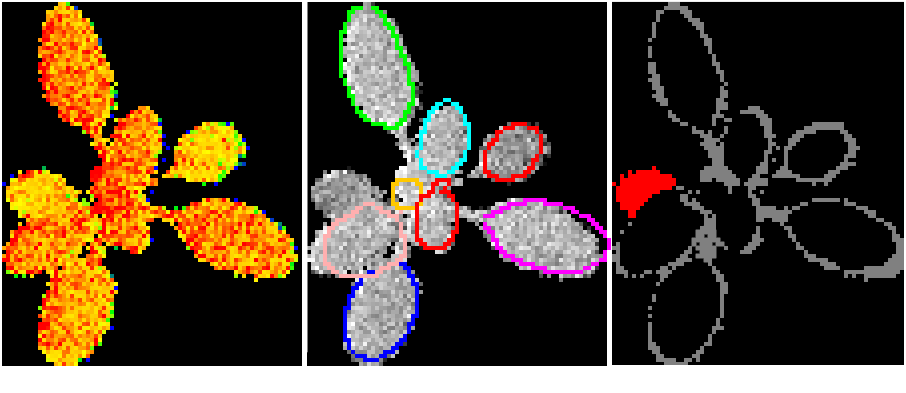
\includegraphics[width=0.45\textwidth]{workflowexample.png}\vspace{-0.2in}
  \caption{An example of the PlantPH workflow, where (a) is a plant image, (b) is leaf alignment results, and (c) is spacial clustering results.}\label{fig:example}\vspace{-0.2in}
\end{figure}

\end{methods}
\section{Results}

We tested the performance of PlantPH on two datasets, i.e. a real dataset from a large-scale Arabidopsis phenotype screen experiment and a synthetic dataset that includes multiple types of heterogeneity patterns. We also compared PlantPH with two popular heterogeneity tests, where one is the traditional Cochran��s Q-test and the $I^2$ statistic, and the other is a grid based heterogeneity test. Overall, the comparisons show that XXX.

\subsection{Arabidopsis Experiment}

\subsubsection{Data Acquisition and Preprocessing}

In the photosynthesis phenotyping experiment, 567 Arabidopsis thaliana plants (wild types and genetic variations with single gene knockout) that include approximately 3,134 individual leaves, were grown side-by-side under three different light conditions (constant, sinusoid, fluctuate), for in total five days from 10 days old from seedling.
%
Top-view fluorescence images were collected periodically (every 15 or 30 minutes) in order to observe the photosynthesis activity of all of the plants simultaneously. Each fluorescence image is a grey-scale image with a resolution of 1M pixels at 12-bit intensity. In total 31,120 fluorescence images were collected. Note that the averaged leaf cell size of Arabidopsis is about $6,000 \mu m^2$ \citep{gegas2014endopolyploidy} and our image resolution is 3,600 pixels per squared inch. Therefore, each pixel in an image is sampled from about 1,000 leaf cells.

To accurately capture photosynthesis activities from the fluorescence images, data preprocessing step was employed to remove image background, identify plants in an image, and delete abnormalities~\citep{xu2015plant}. From all of the processed images,  biologists manually identified all the heterogenous plant images, which serve as the ground truth for performance test.

%The extracted measurements of photosynthesis parameters are presented in the form of multi-dimensional time-series, one dimension for every photosynthesis parameter.

%,
%

%
%Figure ?? shows that the measurements of a photosynthesis parameter $\Phi_{II}$ at one time point are quite different for the leaves of the same plant  (i.e. plant no. 3-7 and 5-5).



\subsubsection{Performance Evaluation}





\subsection{PlantPH on synthetic data}

\subsubsection{Synthetic Data Generation}
A set of synthetic data were generated to test whether $PlantPH$ is properly designed...

%\section{Materials and Methods}


\subsubsection{Performance Evaluation}



% Results and Discussion can be combined.

%\subsection{Outlier detection}
%
%%Three outlier detection methods were adopted to...
%
%An outlier is an observation that appears to deviate markedly from other observations in the sample. Hampel (Hampel, 1971; Hampel, 1974) introduced the concept of the break-down point, as a measure for the robustness of an estimator against outliers.
%%
%The breakdown point is defined as the smallest percentage of outliers that can cause an estimator to take arbitrary large values. Thus, the larger breakdown point an estimator has, the more robust it is. For example, the sample mean has a breakdown point of 1/n, since a single large observation can make the sample mean and variance cross any bound.
%%
%Accordingly, Hampel suggested the median and the median absolute deviation (MAD) as robust estimates of the location and the spread. The Hampel identifier is often found to be practically very effective (Perarson, 2002; Liu et al., 2004).




\section{Discussion}

A consensus view of the data is that the photosynthesis ability of a plant is not uniform across the whole area (Charles 2008, Meng 2007).
%
The photosynthetic properties of plants can vary dramatically across cells, tissues, and organs~\citep{}, reflecting differences in development, stress responses, regulation of processes such as stomatal conductance~\citep{}, photodamage~\citep{}, and storage of photosynthate~\citep{} and contribute substantially to productivity~\citep{}.

For example, we observed that the acclimation of photosynthesis in response to cold temperatures appears to be more rapid and robust in younger or emerging than older leaves, and ecotypes isolated from different latitudes show distinct heterogeneity patterns, implying that these responses are important for adaptation of photosynthesis to fluctuating temperatures.
%
In other cases, exposure of plants to fluctuating light resulted in loss of photosynthetic capacity or increased photoinhibition in specific sets of leaves or leaf sectors. In many cases, older leaves are preferentially affected, suggesting that resources for maintenance or acclimation responses are preferentially directed to younger leaves. However, we have also identified mutant lines where younger leaves are preferentially affected, which presumably affect the development of photosynthetic robustness.

In order to systematically study the leaf level photosynthesis phenotypes, especially in a high-throughput screen manner, we developed a novel computational tool to automatically conduct statistical analysis on leaf based photosynthesis.

In the future, we will consider more plant-specific constraints including leaf shape similarity and symmetry.


\section*{Acknowledgments}\scriptsize
This research was supported by Chemical Sciences, Geosciences and Biosciences Division, Office of Basic Energy Sciences, Office of Science, U.S. Department of Energy (award number DE-FG02-91ER20021) to JC and DMK.

\bibliographystyle{natbib}

\scriptsize
%\bibliographystyle{plain}
\bibliography{heterogeneity}

\end{document}

